\documentclass[UTF8]{ctexart}
\usepackage[T1]{fontenc}
\usepackage{makeidx}
\usepackage{tikz}

\usepackage{graphicx} 
\usepackage{float} 
\usepackage{subfigure} 
\usepackage{booktabs}
\usepackage{amsmath}


\renewcommand\thepage{\zihao{-4} ~\arabic{page}~}
\makeindex
\bibliographystyle{plain}


\begin{document}
\begin{titlepage}
    \centering

    %------------------------------------------------------------
    %    Top rules
    %------------------------------------------------------------

    \rule{\textwidth}{1pt}   % The top horizontal rule
    \vspace{0.2\textheight}  % Whitespace between top horizontal rule and title

    %------------------------------------------------------------
    %    Title
    %------------------------------------------------------------
    \begin{center}
		\quad \\
		\quad \\
		\heiti \fontsize{45}{17} 研究报告
		\vskip 3.5cm
		\heiti \zihao{2}  基于TOPSIS环境评价及空气质量预测
	\end{center}
	% \vskip 3.5cm


    % \vspace{0.025\textheight}   % Whitespace between the title and short horizontal rule

    % \rule{0.83\textwidth}{0.4pt}  % The short horizontal rule under title

    % \vspace{0.1\textheight}  % Whitespace between the short horizontal rule and author

    % %------------------------------------------------------------
    % %    Author
    % %------------------------------------------------------------

    
    % \vfill  % Whitespace between author and date

    % \begin{tikzpicture}
    %    \draw (0,0) sin (1,1) cos (2,0);
    %     \draw (2,0) sin (3,-1) cos (4,0);
    % \end{tikzpicture}
    
    \vfill  % Whitespace between author and date

    {\large \today}
    \vspace{0.1\textheight}  % Whitespace between date and bottom horizontal rule

    %------------------------------------------------------------
    %    Bottom rules
    %------------------------------------------------------------

    \rule{\textwidth}{1pt}  % The bottom horizontal rule

  \end{titlepage}

\newpage


\section{摘要}
随着“绿水青山就是金山银山”战略以及“碳达峰和碳中和”目标的提出,中国要深入贯彻五位一体战略。随着环境监测系统的完备,
如何对监测数据进行良好的挖掘是有效治理环境污染的重要参考。为了研究环境的发展趋势,首先必须对环境质量做出科学的评价,预测其发展趋势,对于实现环境后续保护措施有重要意义。

本文的主要研究内容和创新点如下:


(1)从环境评价模型的普适性推广性出发,利用熵权法解决了传统评价模型各评价指标权重一致、无区分度的问题。利用TOPSIS综合评价模型在很大程度上改进了传统评价方法对指标和数据量要求严苛的局限性,使得软件得的环境评价功能不仅适用于大范围的环境评价也适用于小范围的环境评价,可以实现自然环境评价亦可实现大气环境评价,推广性良好。

(2)以塞罕坝自然环境指标检验软件内环境评价模型对自然环境的普适性,能够很好的评价塞s罕坝地区的自然环境变化趋势,评价结果与塞罕坝环境改善的实际成果相一致。模型检验成果良好,将各省空气污染指标数据导入模型分析,分析结果直观,与实际各省份实际空气质量情况相一致。能为环保部门的后续措施提供参考。

(3)传统环境预测算法往往只使用了单一的空气质量预测模型,难以大范围推广使用,具有一定的局限性。本软件基于灰色预测模型与BP神经网络优缺点,软件嵌入了此两种适用于不同数据量的预测模型。灰色预测模型能充分挖掘较小样本的信息;BP网络能充分挖掘大样本的发展规律。
关键词:环境评价 空气质量预测 TOPSIS综合评价模型 灰色预测 神经网络

\newpage
\tableofcontents
\newpage
\section{问题描述}
随着2020年9月,习近平总书记“中国二氧化碳排放力争于2030年前达到峰值,努力争取2060年前实现碳中和”的发展目标的提出,自然环境、大气环境越来越受到人们的关注.近年来,国内已经出现了许多环境空气质量实时自动检测系统和重点大气污染源的检测系统。

获取监测数据的系统工程已经日趋完善,现代城市环境空气质量管理面临的主要问题是如何有效管理数据资源并挖掘出数据中蕴含的丰富信息,充分发挥信息潜力及价值$^{[1]}$。基于数据信息的挖掘可以为大气环境的评价以及后续的环境指标预测打下坚实的基础。

目前有大量学者提出了关于环境评价和大气污染物、排放物的预测方法。较为主流的评价方法有模糊评价方法;较为主流的预测方法是灰色预测、回归预测和神经网络预测。文献$^{[2]}$提出了模糊评价法在环境评价中的应用,由于环境系统的复杂性,模糊理论的提出有助于降低这种复杂性,模糊理论隶属度的提出很好的降低了指标在系统中的模糊性。文献$^{[3]}$提出一种PLSR回归预测模型,可集成多元线性回归分析,相关性分析和主成分分析,可以很好的解决变量之间存在着多重相关性或样本点过少的回归难题。文献$^{[4]}$也提出利用主成分分析法进行数据降维后的最小二乘回归法,提升了预测精度。文献$^{[5]}$提出了基于灰色系统理论的GM(1,1)预测模型能够挖掘较少数据的发展规律,具有较好的适应性和灵活性。文献$^{[6]}$提出了人工神经网络大气环境数据预测中的应用,人工神经网络具有良好的非线性映射逼近性能,能够充分挖掘大量数据发展规律做出预测。

本文的开发是在大气环境监测系统以及完备的数据统计传输系统已经完备的基础上提出的,目前收集数据的系统已经日趋完备,对于所收集数据进行挖掘,环境的评价,大气指标数据预测的系统还不够完备。为了能够充分利用环境监测系统建立起来的历年监测数据,分析大气环境的变化趋势、对空气质量进行预报,目前有学者对此方面做了一些研究,引进了诸如模糊评价、灰色预测、回归预测、神经网络等对大气数据进行评价预测的方法。对比分析以上学者的研究,总结如下关于各模型的优缺点分析:

针对目前研究的局限性,同时为了建立一个具有普适性的环境评价预测系统,引入了熵权法定权模型,可以消除模糊评价、TOPSIS综合评价法各个权重重要性无区分度的局限性;同时引入TOPSIS综合评价模型。熵权法$^{[7]}$利用熵值来判断某个指标的离散程度,其信息熵值越小,指标的离散程度越大,该指标对综合评价的影响越大,相应的该指标的权重越大。TOPSIS综合评价法$^{[8]}$避免了数据的主观性,不需要目标函数,能够很好的刻画多个影响指标的影响程度;同时TOPSIS综合评价法对数据分布量、指标多少无限制,适用于大样本也适用于小样本,可以适用于多评价单元、多指标的大系统。将两种模型嵌入软件后,不仅可以实现大气环境评价,同时由于TOPSIS模型的普适性,也可以用于其他自然环境指标系统的评价。

同时,以往的模型没有考虑各个模型的适用性,只是单一的预测模型,具有相当的局限性。本文研究过程中,为了满足不同指标、不同数据量的不同用户的使用需求,在软件中嵌入了灰色预测、BP神经网络两种预测模型供用户选择,提高了软件的可塑性,方便用户使用。本软件对模型的优化使得它适用于不同级别的环境部门进行环境数据分析,适用性广泛,能为后续的环保措施提供参考。

\begin{figure}[H] %H为当前位置,!htb为忽略美学标准,htbp为浮动图形
    \centering %图片居中
    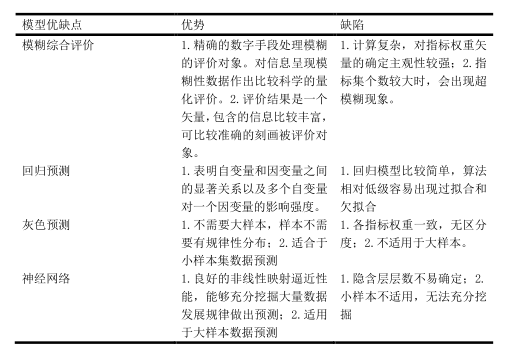
\includegraphics[width=1\textwidth]{./picture/youquedian.png} %插入图片,[]中设置图片大小,{}中是图片文件名
    \caption{各模型优缺点分析} 
\end{figure}

\newpage
\section{模型适用性检验}
\subsection{数据来源}
本文所有的数据均来自国家统计局和地方统计局。
\subsection{数据分析和处理}
由于塞罕坝在过去的几十年间环境改造取得了举世瞩目的成果,本文通过选取塞罕坝环境数据来检验模型的适用性,通过查询国家统计局数据库得到河北市塞罕坝森林覆盖率、森林覆盖面积、林木蓄积、涵养水量、二氧化碳吸收量、氧气释放量6个环境评价指标自1962年至2021年间的完整数据。
首先对获取的塞罕坝数据利用SPSS软件进行描述统计:

\begin{figure}[H] %H为当前位置,!htb为忽略美学标准,htbp为浮动图形
    \centering %图片居中
    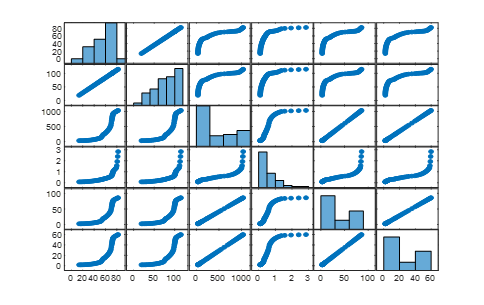
\includegraphics[width=0.7\textwidth]{./picture/datascrip.png} %插入图片,[]中设置图片大小,{}中是图片文件名
    \caption{数据描述统计图} 
\end{figure}


变异系数CV:
\begin{equation}
    CV=\frac{\delta}{\mu}
\end{equation}

其中为样本数据的标准差, 为样本数据的平均值.

当需要比较数据离散程度大小的时候,如果数据的测量尺度相差太大,或者数据量纲的不同,直接使用标准差来进行比较不合适,此时就应当消除测量尺度和量纲的影响,而变异系数可以做到这一点,标准差与其平均数的比。CV虽然没有量纲,同时又按照其均数大小进行了标准化,这样就可以进行客观比较了。因此,可以认为变异系数和极差、标准差和方差一样,都是反映数据离散程度的绝对值。其数据大小不仅受变量值离散程度的影响,而且还受变量值平均水平大小的影响。

当变异系数CV>0.15时,可认为数据中有异常值:

\begin{enumerate}
\item 基于二氧化碳吸收量/万吨,变异系数(CV)为0.875,大于0.15,当前数据中可能存在异常值,建议对异常的或者表现得较为突出的指标进行分析。
\item 基于森林覆盖率,变异系数(CV)为0.344,大于0.15,当前数据中可能存在异常值,建议对异常的或者表现得较为突出的指标进行分析。
\item 基于氧气释放量/万吨,变异系数(CV)为0.875,大于0.15,当前数据中可能存在异常值,建议对异常的或者表现得较为突出的指标进行分析。
\item 基于涵养水量/亿立方米,变异系数(CV)为0.956,大于0.15,当前数据中可能存在异常值,建议对异常的或者表现得较为突出的指标进行分析。
\item 基于覆盖面积/万亩,变异系数(CV)为0.344,大于0.15,当前数据中可能存在异常值,建议对异常的或者表现得较为突出的指标进行分析。
\item 基于林木蓄积/万立方米,变异系数(CV)为0.875,大于0.15,当前数据中可能存在异常值,建议对异常的或者表现得较为突出的指标进行分析。
\end{enumerate}

\subsection{异常值处理}
一组数据只含有随机误差,对其进行计算处理得到标准偏差,按一定概率确定一个区间,认为凡超过这个区间的误差,就不属于随机误差而是粗大误差,含有该误差的数据应予以剔除。这种判别处理原理及方法仅局限于对正态或近似正态分布的样本数据处理,它是以测量次数充分大为前提。根据3 $\sigma$原则。
\begin{equation}
    \text{原则}=\left \{
         \begin{aligned}
            \text{数值分布在(μ-δ,μ+δ)中的概率为0.6826}\\
            \text{数值分布在(μ-2δ,μ+2δ)中的概率为0.9544}\\
            \text{数值分布在(μ-3δ,μ+3δ)中的概率为0.9974}
         \end{aligned}
     \right.
\end{equation}

对样本进行等精度测量,独立得到$x_1,x_2,...,x_n$算出其算术平均值 ,以及剩余误差 ,并计算标准差 ,当样本值 满足:
\begin{equation}
    \left|v_i\right|=\left|x_i-x\right|>3\delta
\end{equation}

则$x_i$应该剔除。据此,筛选出样本中的异常值。对于异常值的处理采用相邻两数据的平均值进行替换。

\begin{figure}[H] %H为当前位置,!htb为忽略美学标准,htbp为浮动图形
    \centering %图片居中
    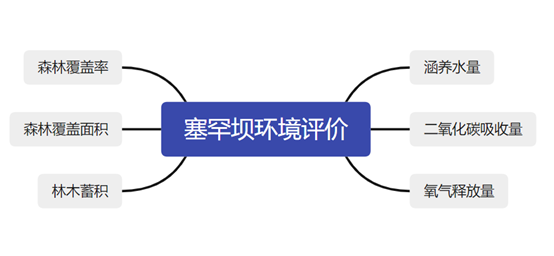
\includegraphics[width=0.7\textwidth]{./picture/saihanbapj.png} %插入图片,[]中设置图片大小,{}中是图片文件名
    \caption{塞罕坝环境评价指标} 
\end{figure}

建立塞罕坝对生态环境的影响评价模型是对评价方法的应用,目前综合评价方法多种多样,如模糊评价法、加权平均法、层次分析法、主成分分析法、熵权评价法、灰色关联评价法、TOPSIS方法和数据包络法等。软件结合熵权法和TOPSIS方法,分析塞罕坝地区改造对环境影响问题。

\newpage
\section{综合评价方法介绍}
\subsection{熵权法}
熵权法是一个客观的赋权方法,可以最大程度上避免主观性赋权对于环境指标量化结果的影响。熵权法权法依据的原理是指标的变异程度,即变异程度越高则对应的权值也就越高。

首先本文需要对环境指标数据进行正向化和归一化处理,保证数据的统一性:
\begin{equation}
    z_{ij}=\frac{x_{ij}-x_{min}}{{xmax}_{max}}
\end{equation}

其中 为归一化处理后的变量,$x_{min}$和 $x_{max}$分别为每个指标的最大值和最值。
计算第j个环境指标下第i个年份所占权重,将其看作计算信息熵时的概率 
\begin{equation}
    p_{ij}=\frac{z_{ij}}{\sum_{i=1}^{n}z_{ij}} 
\end{equation}

计算第j个环境指标的信息熵 ,并计算对应信息效用值 ,此处进行转换的原因是因为信息熵越大代表该环境指标的信息越少,引入 就可以正向衡量信息量。
\begin{equation}
    e_j=-\frac{1}{ln{n}}\sum_{i=1}^{n}{ln{(}p_{ij})}
\end{equation}
\begin{equation}
    d_j=1-e_j
\end{equation}

最终归一化得到每个环境评价指标的熵权$w_j$
\begin{equation}
    w_j=\frac{d_j}{\sum_{j=1}^{m}d_j}
\end{equation}

得到6个权重分别为:

\begin{figure}[H] %H为当前位置,!htb为忽略美学标准,htbp为浮动图形
    \centering %图片居中
    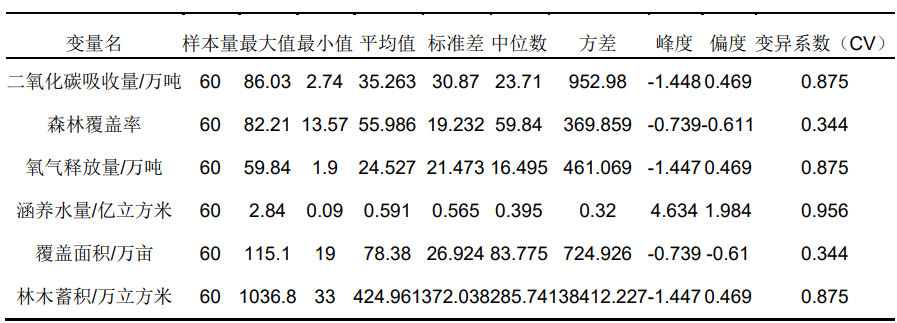
\includegraphics[width=1\textwidth]{./picture/biaoge1.png} %插入图片,[]中设置图片大小,{}中是图片文件名
    \caption{权重表} 
\end{figure}



塞罕坝环境综合评价一项较为复杂的系统工程,在研究此问题时不能忽视指标本身所蕴含的信息。采用了熵权分析法来处理指标权重。按照信息论最基本的原理,信息作为系统有序程度的度量,熵则是系统无序程度的度量,熵权法利用熵值来判断某个指标的离散程度,其信息熵值越小,指标的离散程度越大,该指标对综合评价的影响越大,相应的该指标的权重越大。 
\subsection{TOPSIS综合评价法}
TOPSIS法是用来处理指标决策问题的多方案排序和选择的方法,它的基本思想是:依据理想点的理论原理,找寻距离理想点最近的方案。并通过计算对象与最优解、最劣解的距离大小,确定顺序。即先设定一个虚拟的最优解(又称正理想解)和一个最劣解(又称负理想解),将各备选方案与正负理想解相互比较,若方案最靠近最优解即又距最劣解最远为最好。另外,TOPSIS方法需要的评价指标决策矩阵和指标权重,由上文中的熵权法计算给出。

所选指标均为效益性指标,故不做另外处理。找出每列也就是每个环境指标的最大值,记为$z_i^+(i=1,2,...,m)$ ,组成向量
\begin{equation}
    Z^+={z_1^+,z_2^+,...,z_m^+}
\end{equation}

该向量代表了环境最好的年份。同样的,找出每列也就是每个指标的最小值,记为$z_i^-(i=1,2,...,m)$ ,组成向量

\begin{equation}
    Z^-={z_1^-,z_2^-,...,z_m^-}
\end{equation}

该向量代表了环境最差的年份。

定义第i个年份与理想目标距离为$D_i^+$ ,计算公式为
\begin{equation}
    D_i^+=\sqrt{\sum_{j=1}^{m}{w_j(z_j^+-z_{ij})^2}}
\end{equation}

定义第i个年份与不理想目标距离为$D_{ij}^-$,计算公式为
\begin{equation}
    D_i^+=\sqrt{\sum_{j=1}^{m}{w_j(z_j^+-z_{ij})^2}}
\end{equation}

定义第i个年份的得分为$S_i$,计算公式为
\begin{equation}
    S_i=\frac{D_i^-}{D_i^++D_i^-}
\end{equation}
显然,$S_i\in[0,1]$当$S_i$越接近于1,说明此年份i距离理想化目标越近,该年份塞罕坝环境就越好。反之,当 越接近于0,说明年份i距离理想化目标越远,该年份塞罕坝环境就越差。

\newpage
将两种算法嵌入分析系统后,设计如图所示的操作界面:

\begin{figure}[H] %H为当前位置,!htb为忽略美学标准,htbp为浮动图形
    \centering %图片居中
    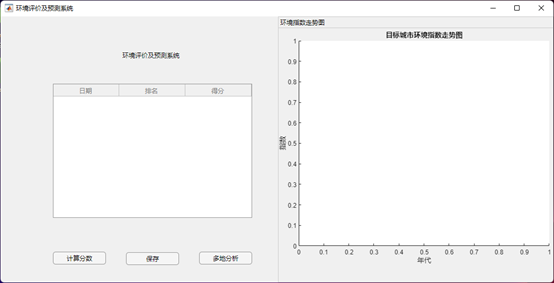
\includegraphics[width=0.7\textwidth]{./picture/caozuojiemian1.png} %插入图片,[]中设置图片大小,{}中是图片文件名
    \caption{评价操作界面} 
\end{figure}

将数据导入分析系统得到1962-2021年间塞罕坝环境的量化得分:

\begin{figure}[H] %H为当前位置,!htb为忽略美学标准,htbp为浮动图形
    \centering %图片居中
    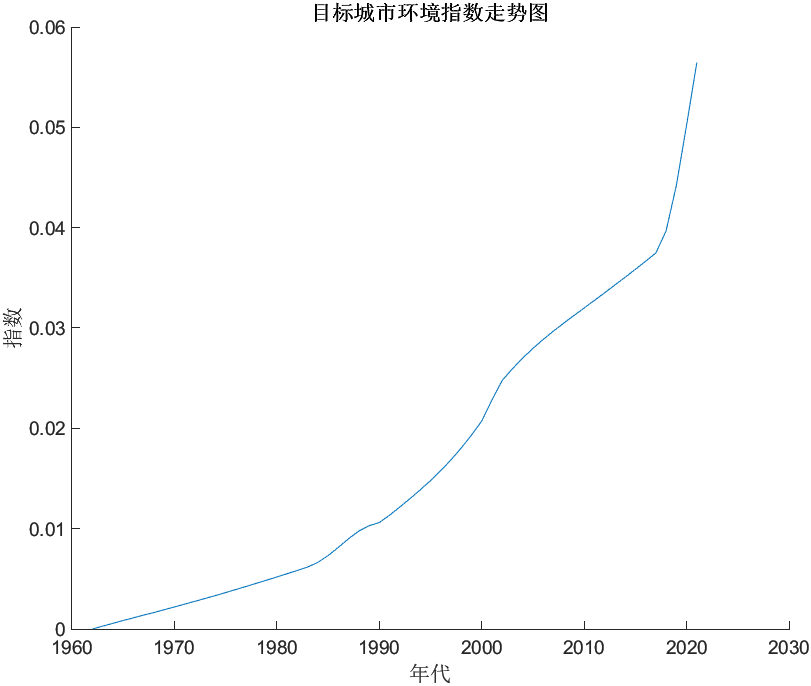
\includegraphics[width=0.7\textwidth]{saihanba.png} %插入图片,[]中设置图片大小,{}中是图片文件名
    \caption{塞罕坝评价历年环境指数} 
\end{figure}

根据评价模型得出的1962年到2021年塞罕坝环境得分呈上升趋势,可知塞罕坝恢复对环境改造有积极作用。塞罕坝几代人的防沙治沙卓有成效,不仅留下了巨大精神财富,也为后来环境改造工程提供了范本。

\section{大气环境综合评价}
目前全国的环境保护监测站已经建立起一套十分完备的城市环境质量监测系统,包括空气质量实时监测系统和重点污染源在线监控系,使得全国各地的空气质量监测数据都能通过系统上传到城市环境空气质量数据库$^{[9]}$最终被国家统计局收录,本文从国家统计局官网下载2021年12月各个市份PM2.5、PM10、AQI(空气质量指数)作为评价指标数据来研究软件中模型的适用性。

\subsection{PM2.5浓度和PM10}
大气污染物因子有很多种,当前我国环境保护部门监测环境空气污染物时采用的是PM10这个指标。其定义是监测环境空气中尘埃或飘尘的空气当量直径为10μm的尘埃或飘尘在环境空气中的浓度$C_{PM2.5}$。由此,就知道了PM2.5,就是指:直径小于或等于2.5μm的尘埃或飘尘在环境空气中的浓度$C_{PM2.5}$。PM2.5和PM10的主要成分包括:含碳颗粒(包括元素碳和有机碳,元素碳主要产生于高温燃烧过程,有机碳则主要来自相对低温过程的不完全燃烧产物)、硫酸盐、硝酸盐、铵盐、重金属等。PM2.5和PM10在空气悬浮过程中还会进一步吸附空气中存在的有机和金属等化学成分、细菌、病毒、真菌等微生物成分。对空气质量破坏明显,对人体危害极大。

\subsection{AQI(空气质量指数)}
空气质量指数(Air Quality Index,简称AQI),是一个用来定量描述空气质量水平的数值。AQI的取值范围位于0-500 之间。环境空气污染物的种类有很多,参与AQI指数评价的有二氧化硫(SO2)、二氧化氮(NO2)、一氧化碳(CO)、臭氧(O3)、PM2.5、PM10。

\begin{figure}[H] %H为当前位置,!htb为忽略美学标准,htbp为浮动图形
    \centering %图片居中
    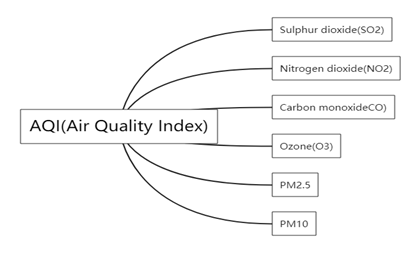
\includegraphics[width=0.7\textwidth]{./picture/AQI.png} %插入图片,[]中设置图片大小,{}中是图片文件名
    \caption{AQI评价指标内容} 
\end{figure}

环境监测部门每天发布的空气质量报告中,会包含各种污染物的浓度值。很难从这么多个抽象的浓度数据中判断出到底当前的空气质量处在什么水平。于是将各种不同污染物含量折算成一个统一的指数,这就是空气质量指数。 空气质量指数的值在不同的区间,就代表了不同的空气质量水平。比如0-50之间,代表良好;51-100之间,代表中等;101-150之间代表轻度污染等等。为了更直观起见,每个区间都有一个固定的颜色值与它对应:

\begin{figure}[H] %H为当前位置,!htb为忽略美学标准,htbp为浮动图形
    \centering %图片居中
    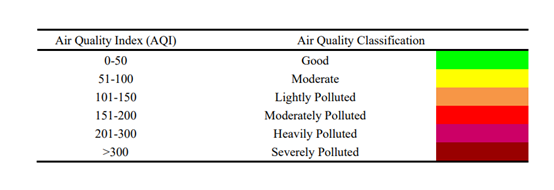
\includegraphics[width=0.9\textwidth]{./picture/biaoge2.png} %插入图片,[]中设置图片大小,{}中是图片文件名
    \caption{AQI数据对应表} 
\end{figure}

AQI的折算公式如下:
\begin{equation}
    I=\frac{I_{high}-I_{low}}{C_{high}-C_{low}}(C-C_{low})+I_{low}
\end{equation}

其中I等于空气质量指数,即AQI,输出值;C为污染物浓度,输入值;$C_{low}$为小于或等于C的浓度限值$C_{high}$为大于或等于C的浓度限值;$I_{low}$对应于$C_{low}$的指数限值;$I_{high}$为对应于$C_{high}$的指数限值

多地分析过程中往往需要对比分析,基于此本软件设计了多地分析按钮,具体模型沿用上文中的综合评价模型,嵌入了条形统计分析图,箱线图等统的计学分析图表功能。将搜集数据带入计算,得到如下结果:

\begin{figure}[H] %H为当前位置,!htb为忽略美学标准,htbp为浮动图形
    \centering %图片居中
    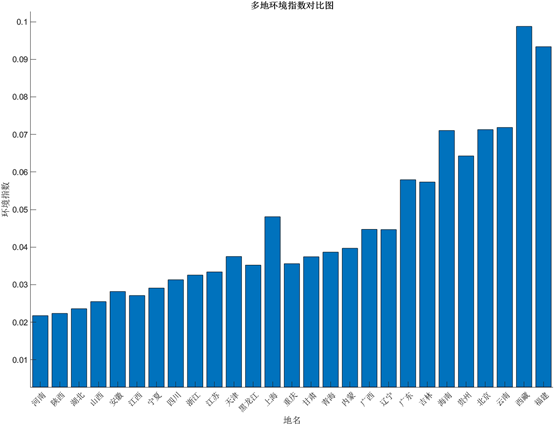
\includegraphics[width=0.6\textwidth]{./picture/geshengpaiming.png} %插入图片,[]中设置图片大小,{}中是图片文件名
    \caption{空气质量评价结果热力图} 
\end{figure}

利用Matlab编程得到环境质量指数热力图,将各个省份的数据可视化后,可以看出我国南方地区普遍空气质量较好。
除开天津沙漠的原因导致的气候异常,华北平原和华中平原目前属于环境空气污染较为严重的地区。
\begin{figure}[H] %H为当前位置,!htb为忽略美学标准,htbp为浮动图形
    \centering %图片居中
    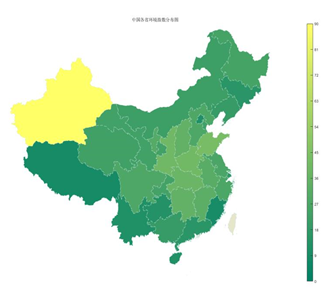
\includegraphics[width=0.85\textwidth]{./picture/renlitu.png} %插入图片,[]中设置图片大小,{}中是图片文件名
    \caption{全国环境质量指数热力图} 
\end{figure}

\newpage
\section{环境变化预测分析}
为了预测天津市后续三月的环境变化趋势,通过前文的数据获取、存储方式从国家统计局数据库搜集天津市2014-2021各年的气象AQI指数、PM2.5指数、PM10指数数据。为了让用户直观的观察环境变化趋势,本系统利用二次拟合将数据变化趋势直观的体现给用户,对数据的变化趋势预测,大致反映了后续变化规律,导入数据后,会出现相应指标的变化趋势。下图为天津市PM2.5,PM10,AQI指标的趋势。
\begin{figure}[H] %H为当前位置,!htb为忽略美学标准,htbp为浮动图形
    \centering %图片居中
    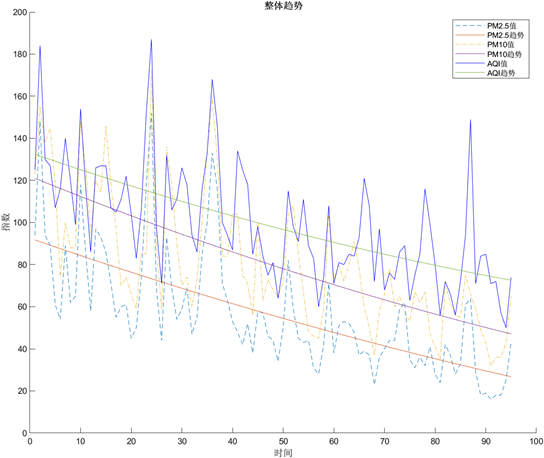
\includegraphics[width=0.9\textwidth]{./picture/PM2.5.png} %插入图片,[]中设置图片大小,{}中是图片文件名
    \caption{PM2.5,PM10,AQI趋势图} 
\end{figure}
可以看到天津市的PM2.5,PM10,AQI整体都趋于下降。

\subsection{BP神经网络模型设计}
首先利用上文的归一化公式进行数据处理,方便进行后面的数据处理,同时保证程序运行时的收敛速度。

对数据归一化处理后,初始化BP神经网络时需要根据系统输入、输出序列(X,Y)来确定输入层节点数量、隐含层节点数量、输出层节点数量、目标误差、迭代次数。在对数据特征进行分析后,本系统设定神经网络允许精度 ,最大学习次数 ,隐含层层数为2层,隐含层每层神经元数量为5个,由此建立了如图所示的神经网络结构:
\begin{figure}[H] %H为当前位置,!htb为忽略美学标准,htbp为浮动图形
    \centering %图片居中
    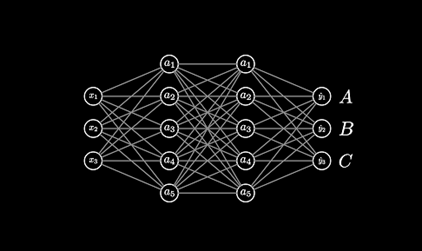
\includegraphics[width=0.7\textwidth]{./picture/network.png} %插入图片,[]中设置图片大小,{}中是图片文件名
    \caption{神经网络结构} 
\end{figure}


隐含层传输函数采用sigmod函数:
\begin{equation}
    f(x)=\frac{1}{1+e^{-x}}
\end{equation}

搭建好神经网络模型后,计算得到计算了将来三个月各项空气指标的变化。
\begin{figure}[H] %H为当前位置,!htb为忽略美学标准,htbp为浮动图形
    \centering %图片居中
    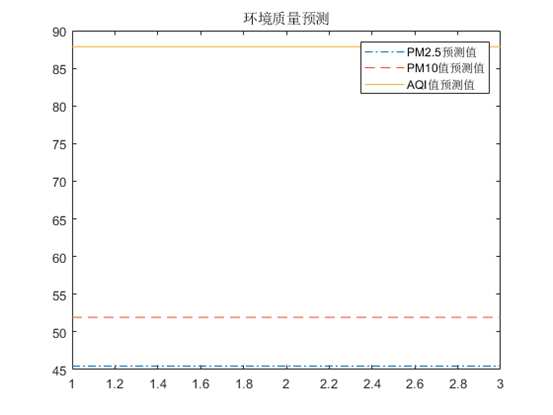
\includegraphics[width=0.7\textwidth]{./picture/sjwl2.png} %插入图片,[]中设置图片大小,{}中是图片文件名
    \caption{将来三个月空气指标神经网络预测} 
\end{figure}

\subsection{灰色预测模型}
灰色预测模型进行预测对原始数据进行累加生成,得到近似的指数规律在进行建模。能够利用微分方程充分挖掘系统的本质,精度高;能够将无规律的的原始数据进行生成得到规律性较强的生成序列:
\begin{equation}
    x^{(0)}=(x^{(0)}(1),x^{(0)}(2),...,x^{(0)}(n))
\end{equation}

一次累加生成序列:
\begin{equation}
    x^{(1)}=(x^{(1)}(1),x^{(1)}(2),...,x^{(1)}(10))=(x^{(0)}(1),x^{(0)}(1)+x^{(0)}(2),...x^{(0)}(1)+...+x^{(0)}(n))
\end{equation}

式中:
\begin{equation}
    x^{(1)}(k)=\sum_{i=1}^{k}{x^{(0)}(i),k=1,2,...,n}
\end{equation}

$x^{(1)}$的均值生成序列:
\begin{equation}
    z^{(1)}=(z^{(1)}(2),z^{(1)}(3),...,z^{(1)}(n))
\end{equation}

式中:
\begin{equation}
    z^{(1}(k)=0.5x^{(1)}(k)+0.5x^{(1)}(k-1),k=2,3,...n
\end{equation}

建立灰微分方程:
\begin{equation}
    x^{(0)}(k)+az^{(1)}(k)=b,k=2,3,...,n
\end{equation}

相应的白化微分方程为:
\begin{equation}
    \frac{dx^{(1)}}{dt}+ax^{(1)}(t)=b
\end{equation}

记
\begin{equation}
    u=\left[a,b\right]^T
\end{equation}

\begin{equation}
    Y=[x^{(0)}(2),x^{(0)}(3),...,x^{(0)}(n)^T]
\end{equation}

% \begin{equation}
%     B=\left[\begin{matrix}-z^{(1)}(2)&1\\-z^{(1)}(3)&1\\...&...\\-z^{(1)}(10)&1\\\end{matrix}\right]
% \end{equation}

则由最小二乘法,求得使$J(u)=(Y-Bu)^T(Y-Bu)$达到最小值的u的估计值为

\begin{equation}
    \hat{u}=[\hat{a},\hat{b}]T=(BTB)-1BTY
\end{equation}

于是得到方程:
\begin{equation}
    \hat{x}(k+1)=(x^{(0)}(1)-\frac{\hat{b}}{\hat{a}})e^{-\hat{a}k}+\frac{\hat{b}}{\hat{a}},k=0,1,...,n 
\end{equation}

灰色预测模型运作时,需要对已知数据进行必要的级比检验,参考数据$x^{(0)}=(x^{(0)}(1),x^{(0)}(2),...,x^0(n))$,计算序列的级比:
\begin{equation}
    \lambda(k)=\frac{x^{(0)}(k-1)}{x^{(0}(k)},k=2,3,...n, 
\end{equation}

当计算得到的级比$\lambda(k)$都落在可容覆盖$\theta$内$x^{(0)}$序列 可以作为模型$GM(1,1)$的数据进行预测。

将数据导入模型,计算得:
\begin{figure}[H] %H为当前位置,!htb为忽略美学标准,htbp为浮动图形
    \centering %图片居中
    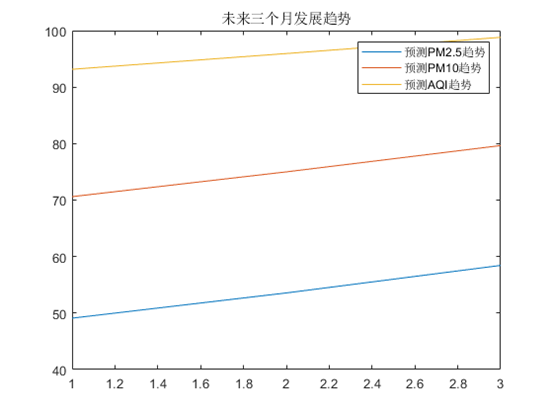
\includegraphics[width=0.7\textwidth]{./picture/hsyc2.png} %插入图片,[]中设置图片大小,{}中是图片文件名
    \caption{未来三个月指标灰色预测} 
\end{figure}s

未来三个月PM2.5、PM10及AQI的值分别在90到100,70到80,50到60左右。

\newpage
\section{天津市空气污染治理状况及对策}
搜集天津2000-2020年废气治理财政支出,绘制如下的走势图:

\begin{figure}[H] %H为当前位置,!htb为忽略美学标准,htbp为浮动图形
    \centering %图片居中
    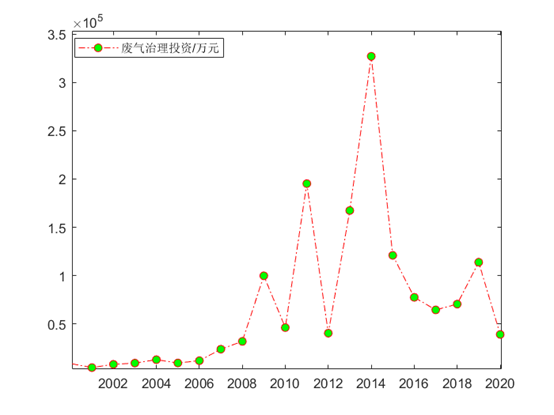
\includegraphics[width=0.7\textwidth]{./picture/touzi.png} %插入图片,[]中设置图片大小,{}中是图片文件名
    \caption{天津废气治理投资} 
\end{figure}

可以看出,天津近几年在废气治理投入较少,着眼于双碳目标同时为了遏制大气环境的恶化,应及时增加废气治理的投资。

根据空气质量预测走势图可以得出,出现一个大的峰值的周期大概在12个月,小波峰的周期大概是3个月,在每年的冬季是空气质量最差的季节,由于供暖和更多的私家车上路,造成空气污染更为严重。应对此种现象,可以考虑采用清洁能源取暖,减少燃煤取暖;同时在冬季来临之前的三个月内提前适当限行车辆,减少尾气排放。为了遏制天津空气质量的恶化,后续应重点控制电力、热力生产企业、黑色金属、有色金属行业的废气排放量。
\newpage
其中电力行业产生的废气多的原因主要是由于我国的新能源装机容量不足,截至2020年底,全国电源总装机容量超过22亿千瓦,火电水电仍为第一第二大电源,分别占比57\%,17\%。当前电力行业二氧化碳排放约占中国能源活动二氧化碳排放的40\%。2020年全社会用电量为7.5万亿千瓦时,十三五期间全社会用电量年均增速为5.7\%。利用新能源代替传统发电仍需继续研究,逐步推进。拉闸限电势在必行。对于相关部门而言,应加大重点行业排放的监督力度,引导企业做好生产后的废气净化处理,加大投入。减少火力发电,引进新能源发电技术迫在眉睫。
\begin{figure}[H] %H为当前位置,!htb为忽略美学标准,htbp为浮动图形
    \centering %图片居中
    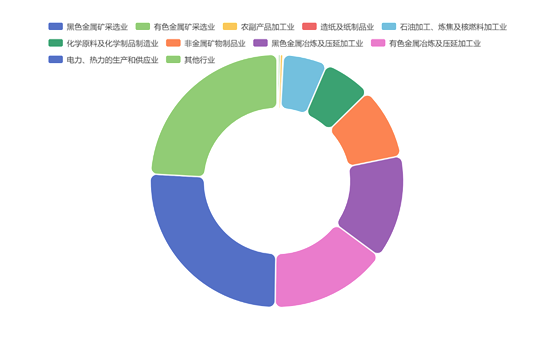
\includegraphics[width=1\textwidth]{./picture/quanquan.png} %插入图片,[]中设置图片大小,{}中是图片文件名
    \caption{各行用电占比} 
\end{figure}

\newpage
\section{研究结论总结}
基于TOPSIS的环境评价空气质量预测系统的开发对大气质量的评价预测具有一定意义。研究着眼于环境质量评价方法、空气质量预测方法现状,分析了国内研究进展和目前环境评价预测系统的不足。

\begin{figure}[H] %H为当前位置,!htb为忽略美学标准,htbp为浮动图形
    \centering %图片居中
    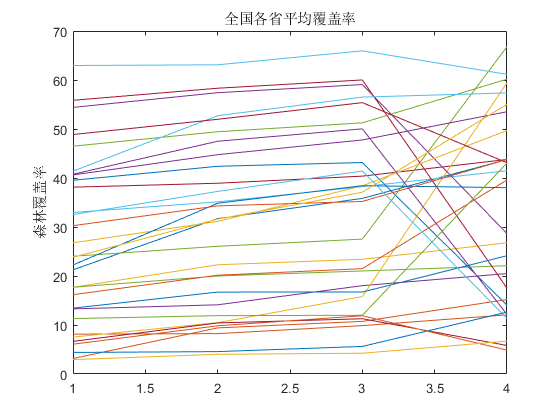
\includegraphics[width=0.9\textwidth]{./picture/geshenglsf.png} %插入图片,[]中设置图片大小,{}中是图片文件名
    \caption{近四次全国森林覆盖率} 
\end{figure}

\begin{figure}[H] %H为当前位置,!htb为忽略美学标准,htbp为浮动图形
    \centering %图片居中
    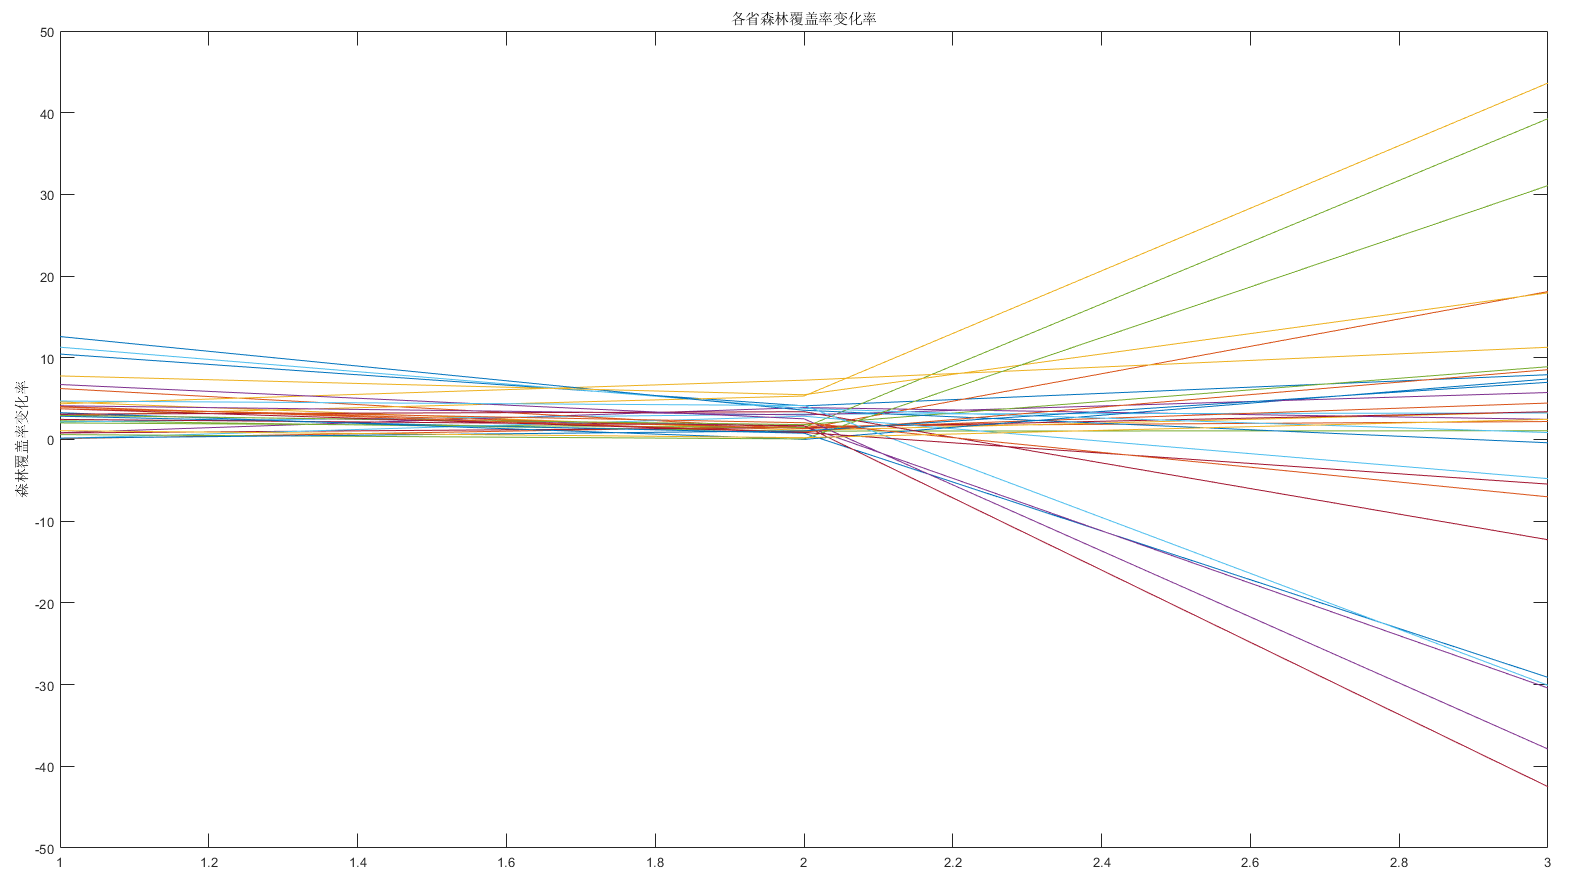
\includegraphics[width=1\textwidth]{./picture/newrate.png} %插入图片,[]中设置图片大小,{}中是图片文件名
    \caption{近四次全国森林覆盖率变化率} 
\end{figure}
本文以matlab2019、SPSS等软件作为分析工具,软件界面简洁、使用便捷,能满足不同用户的操作需求。

在进行环境质量评价的过程中,为了消除传统评价方法不同数据量、数据类型的局限性,提出了具有普适性的TOPSIS综合评价模型,并利用熵权法挖掘各指标的重要程度、解决了传统评价方法指标无区分度的问题。在进行空气质量预测过程中,软件同时嵌入了灰色预测、BP神经网络两个预测模型。灰色预测模型擅长挖掘小样本的发展规律,对于小型区域的空气指标数据预测具有良好效果,小地区上的环境部门可使用此预测模型。BP神经网络能够挖掘大样本的发展规律,适用于大片区域的环境评价预测,能够为全国范围内的后续环保措施提供参考。

软件在检验过程中几个模型均表现良好,基于两种算法的耦合评价模型具有良好的普适性,可以推广到不同级别环境部门进行使用分析。近年“绿水青山就是金山银山”政策以及“碳达峰、碳中和”目标的提出,越来越多的学者、专家将目光投入环境评价和预测中去。随着计算机技术的发展,待更多的优秀的评价预测算法的出现,可把大气环境评价预测推进到一个更高的水平。

\newpage
\section{参考文献}
[1]李丽. 基于数据挖掘的城市环境空气质量决策支持系统设计与实现[D].山东师范大学,2006.

[2]马媛媛,孙世群.模糊综合评价在合肥市大气环境评价中的应用[J].环境科学与管理,2012,37(05):188-191.

[3]王刚,张福印,李明辉,王金龙,王艺博,武传伟.基于偏最小二乘回归算法的空气质量监测系统研究[J].传感器与微系统,2022,41(01):37-40+49.DOI:10.13873/J.1000-9787(2022)01-0037-04.

[4]金文彪,姚永杰,金哲植.基于主成分分析的大气环境预测研究[J].科教导刊(中旬刊),2016(32):148-150.DOI:10.16400/j.cnki.kjdkz.2016.11.071.

[5]李力争,李淑民,张晓郁,赵立娜.灰色系统在大气环境质量评价及变化趋势研究中的应用[J].环境科学与管理,2013,38(01):177-180.

[6]邬红娟,林子扬,郭生练.人工神经网络方法在资源与环境预测方面的应用[J].长江流域资源与环境,2000(02):237-241.

[7]袁冲.基于熵权法的江苏省各市经济高质量发展评价分析[J].商业经济,2022(04):19-20+42.DOI:10.19905/j.cnki.syjj1982.2022.04.061.

[8]徐政华,曹延明.基于熵权TOPSIS模型的长春市水资源承载力评价[J/OL].安全与环境学报:1-10[2022-03-27].DOI:10.13637/j.issn.1009-6094.2021.1448
\end{document}